
\noindent\begin{minipage}{\textwidth}
    \begin{table}[H]
        \centering
        \caption{Hiperparâmetros e Resultados do Melhor Modelo - convnext\_v9\_AM\_opt\_aug}
        \vspace{0.2cm}
        \resizebox{\textwidth}{!}{%
            \begin{tabular}{ll | lrrr}
                \hline
                \multicolumn{2}{c|}{\textbf{Hiperparâmetros}} & \multicolumn{4}{c}{\textbf{Métricas por Classe}} \\ \hline
                \textbf{Parâmetro} & \textbf{Valor} & \textbf{Classe} & \textbf{Precisão} & \textbf{Recall} & \textbf{F1-Score} \\ \hline
    Agendador (Patience) & 5 & 31.2 & 0,7230 & 0,6814 & 0,7016 \\ 
Agendador de LR & ReduceLROnPlateau & 31.3 & 0,5990 & 0,5990 & 0,5990 \\ 
Architecture & convnext\_tiny & 31.4 & 0,4925 & 0,6238 & 0,5504 \\ 
Batch Size & 32 & 32.3 & 0,6923 & 0,6429 & 0,6667 \\ 
Data Augmentation & False & 32.4 & 0,8636 & 0,3276 & 0,4750 \\ 
Decaimento de Peso (WD) & 0,0161 & 33.3 & 0,6048 & 0,7772 & 0,6803 \\ 
Dropout & 0,3037 & 41.4 & 0,6667 & 0,4091 & 0,5070 \\ 
Função de Perda & CrossEntropyLoss & 41.5 & 0,8333 & 0,7692 & 0,8000 \\ 
Hidden Units & 512 & 42.4 & 0,7727 & 0,5000 & 0,6071 \\ 
Label Smoothing & 0,1604 & 44.4 & 1,0000 & 0,8621 & 0,9259 \\ 
\cline{3-6} 
Otimizador & AdamW & \textbf{Média (Macro)} & 0,7247 & 0,6249 & 0,6531 \\ 
Taxa de Aprendizado (LR) & 1,17e-04 & \textbf{MCC} & \multicolumn{3}{c}{0,5809} \\ 
Unfreeze Layers & 3 &  & & &  \\ 
            \hline
            \end{tabular}%
        }
    \end{table}

    \begin{figure}[H]
        \centering
        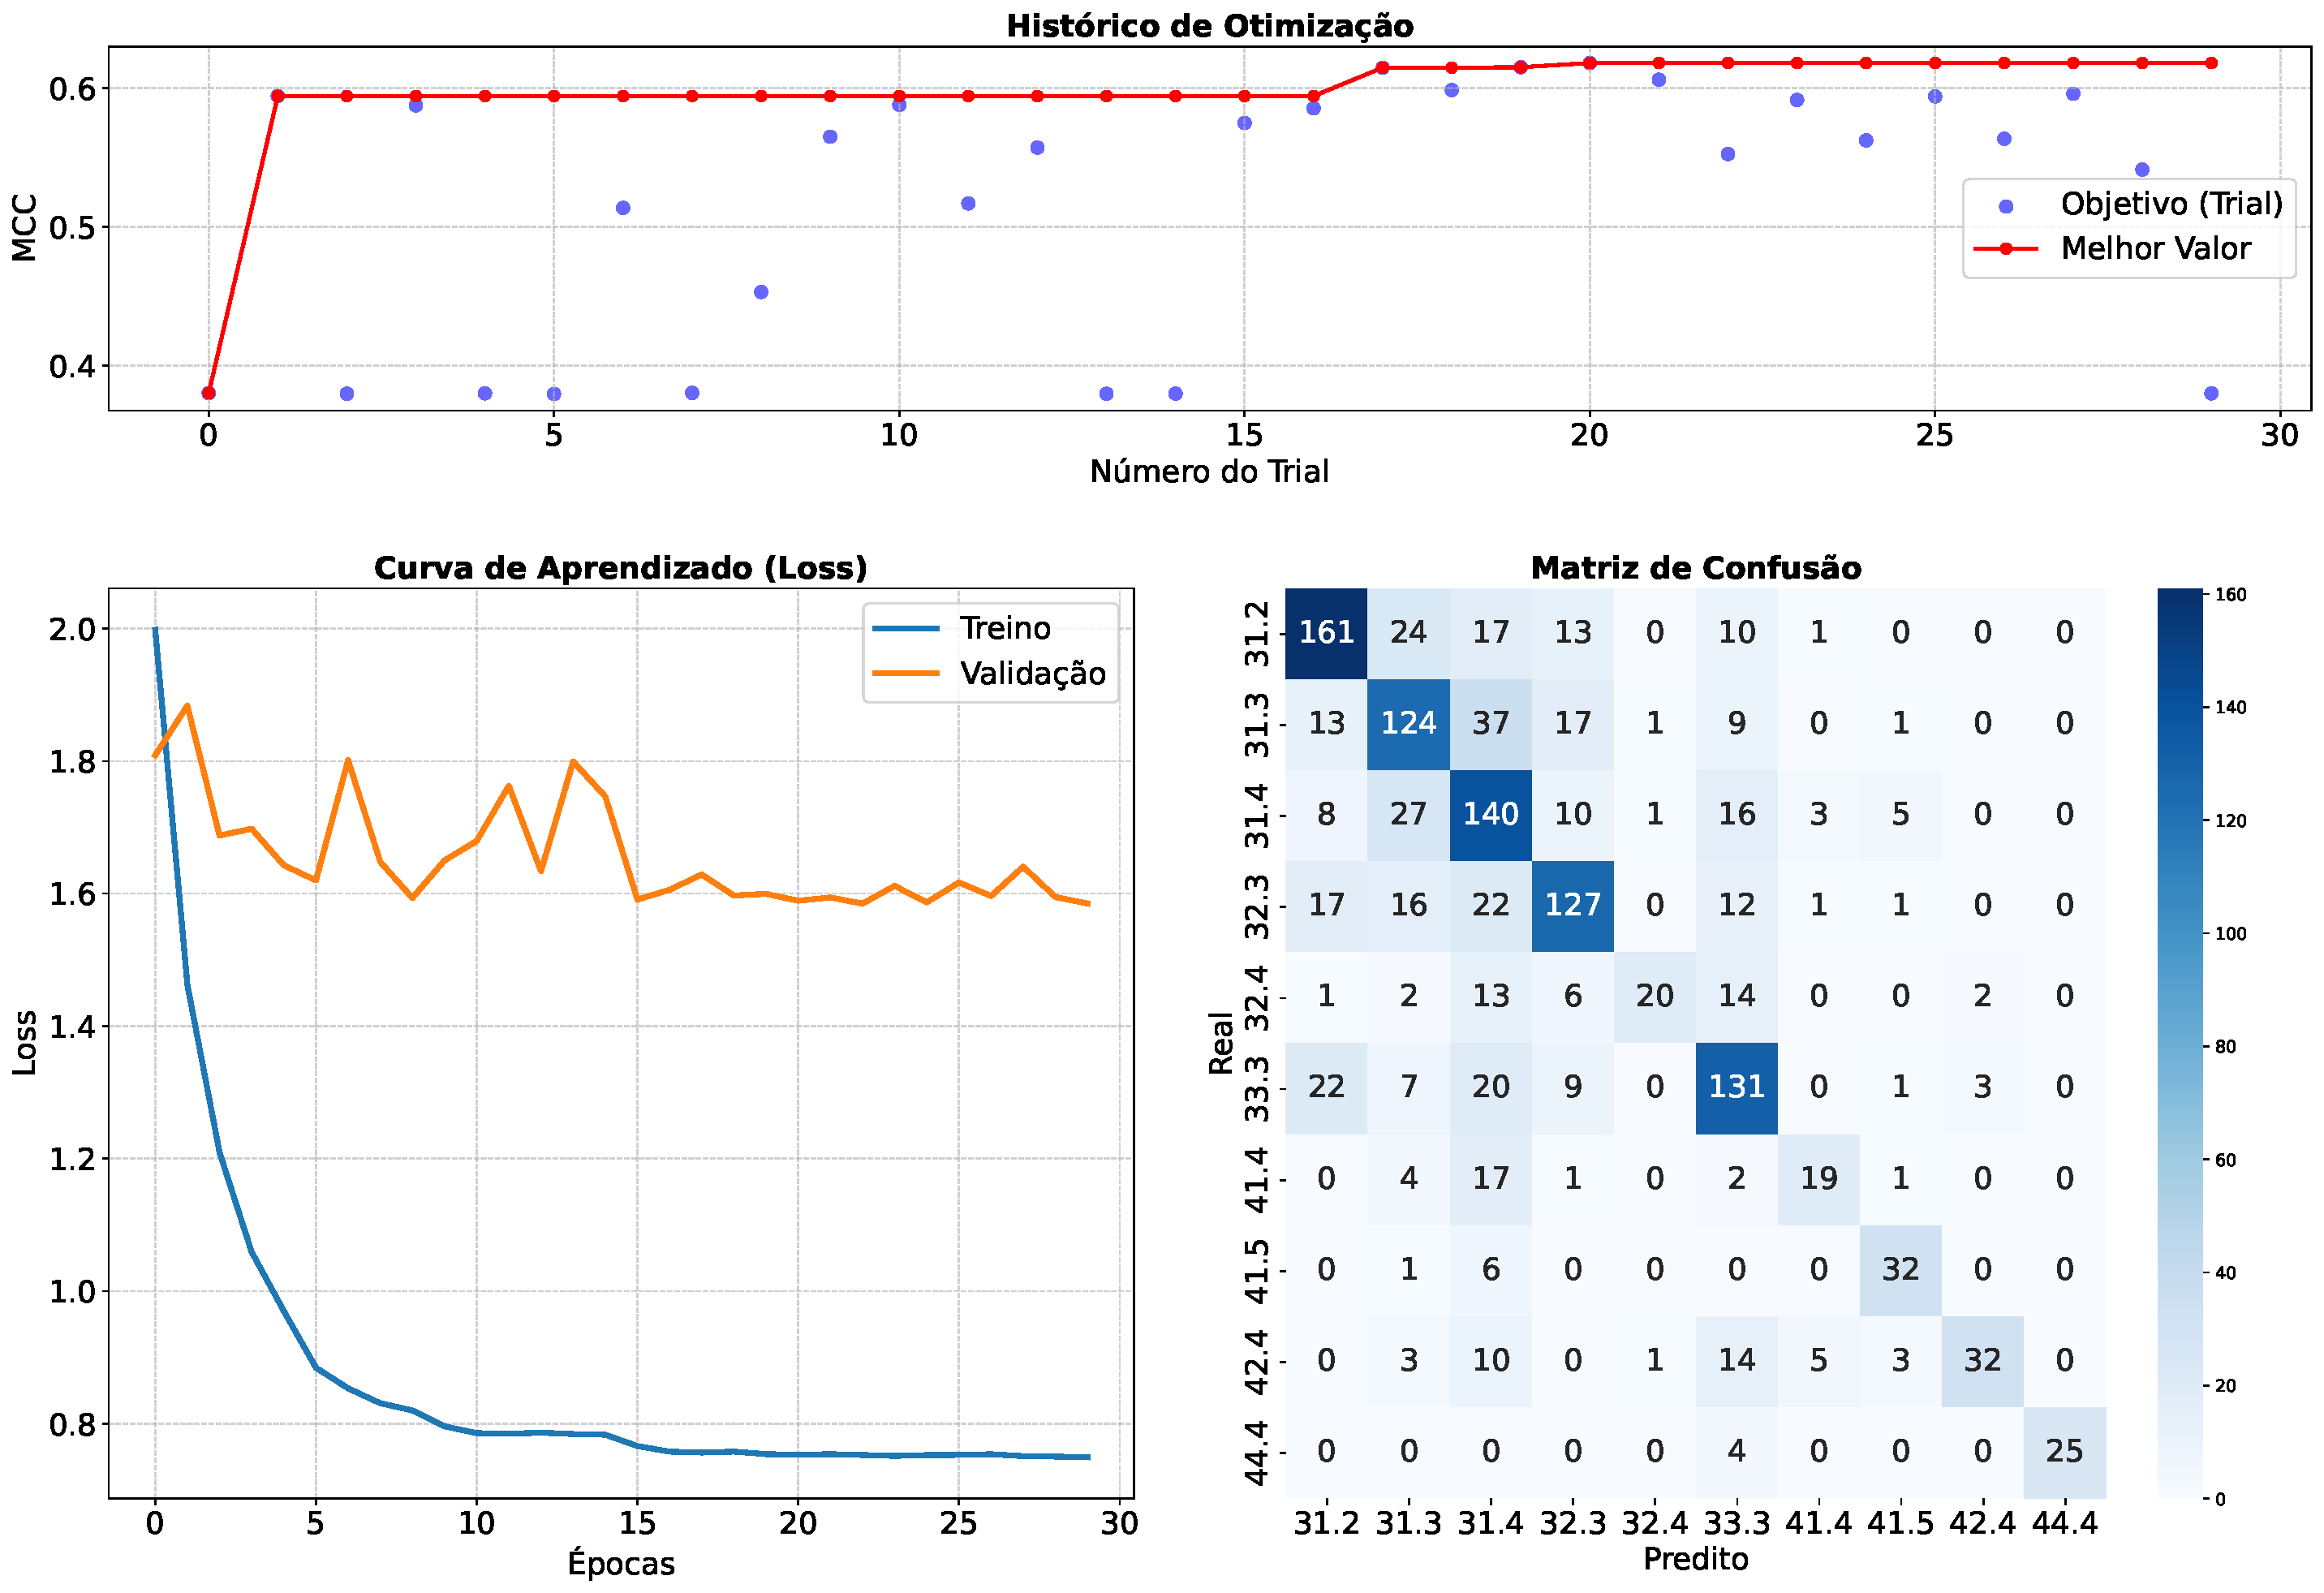
\includegraphics[width=0.85\textwidth]{tex/appendix/experiments/convnext_v9_AM_opt_aug/dashboard_consolidado.pdf}
        \caption{Histórico de Otimização, Curvas de Aprendizado e Matriz de Confusão - convnext\_v9\_AM\_opt\_aug}
    \end{figure}
\end{minipage}
\clearpage
